\FloatBarrier
\begin{figure}[!h]
\centering
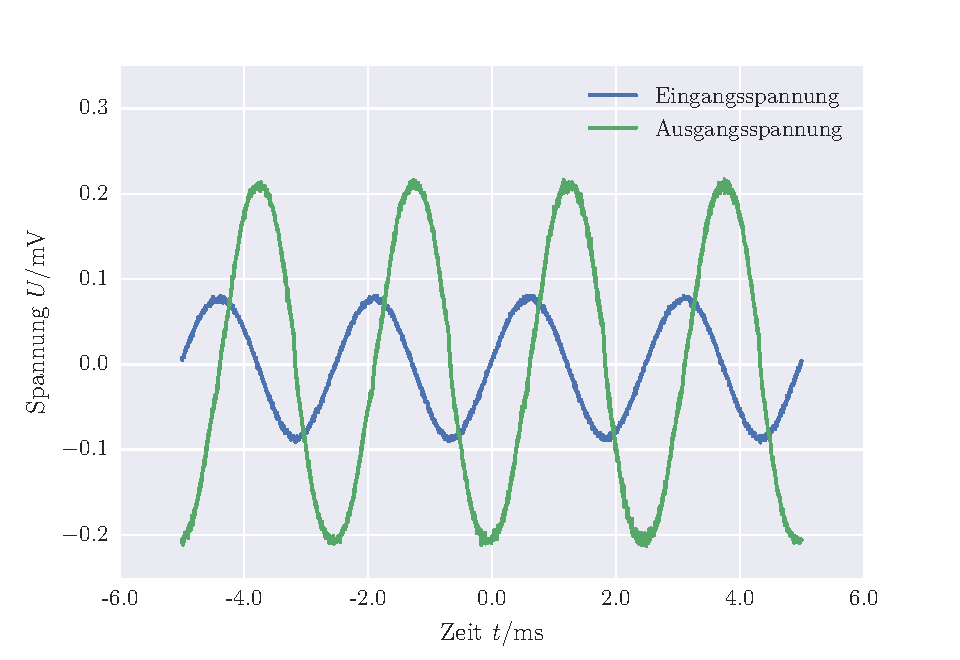
\includegraphics[scale=0.75]{../Grafiken/Differentiator_Oszilloskop_Sinus.pdf}
\caption{Vom Oszilloskop aufgenommene Ein- und Ausgangsspannungen der Differentiatorschaltung. Auf dem Eingang
	liegt hier eine Sinusspannung. Die Ausgangsspannung in Form eines (negativen) Kosinus entspricht dem theoretisch
	zu erwartendem Verlauf.\label{fig:differentiator_oszilloskop_sinus}}
\end{figure}
\FloatBarrier